\chapter{Application Technical Description} \label{chr:appTechDescription}

The objective of this thesis is to extend an existing open-source application, named \emph{dose3d}, which provides a comprehensive set of ready-to-use tools that are beneficial in the field of radiation therapy. The development comprises the creation of two modules: one enabling the W-L test and the other enabling leaves alignment analysis. A theoretical description of the modules can be found in \autoref{chr:wlTest} and \autoref{chr:laModule}, respectively. This chapter describes the application, its design, and its implementation, divided into frontend and backend.

\section{Frontend}

\subsection{UI}

\subsubsection{Structure}

The tabs containing links to both modules can be found on the side panel in the modules section - \autoref{fig:uiLeftPanel}. Each module consists of two pages - a setup page and a results page. The setup page contains a form, where the user can specify input data and two buttons, one for submitting the form and the other for aborting operation. All fields need to be filled in to proceed, otherwise the submit button will be disabled. When a form is submitted, the algorithm is executed and the results are displayed on the results page.

\begin{figure}
    \centering
    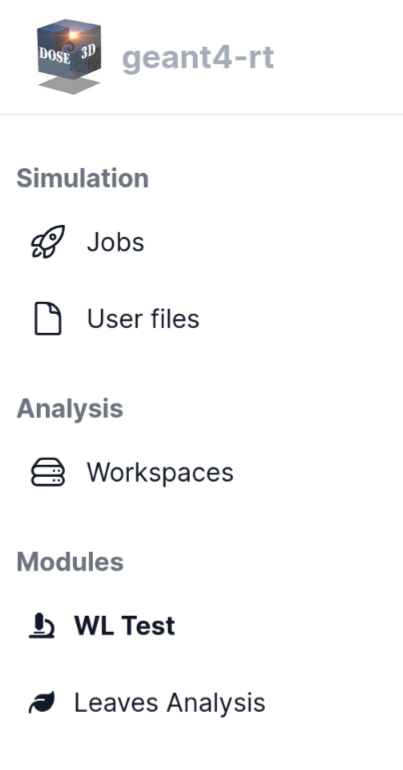
\includegraphics[width=0.30\textwidth]{Content/Images/ui_left_panel.png}
    \caption{Side panel with links to application modules}
    \label{fig:uiLeftPanel}
\end{figure}

\subsubsection{W-L test setup page}

The W-L test setup page consists of two inputs, one numerical for specifying BB size, and the other one for files. Only the zip file can be selected. Once the file has been uploaded correctly, the field will be highlighted in green. W-L setup page is shown on \autoref{fig:uiWLSetup}.

\begin{figure}
    \centering
    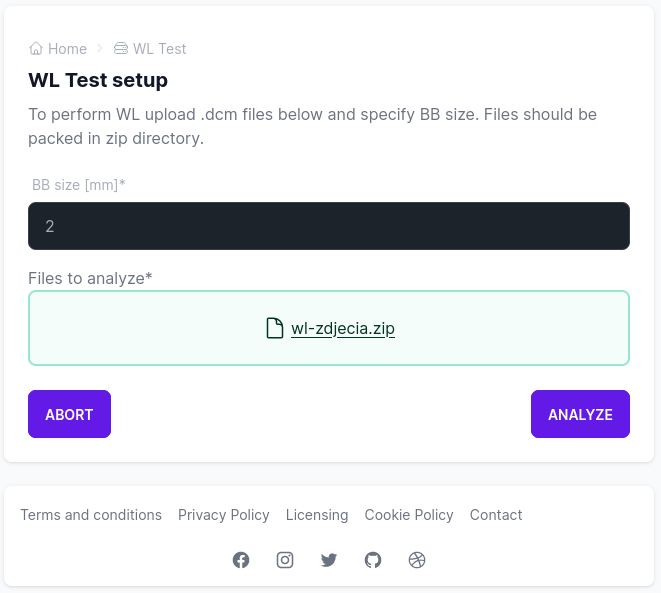
\includegraphics[width=0.6\textwidth]{Content/Images/ui_wl_setup_page.png}
    \caption{W-L test setup page}
    \label{fig:uiWLSetup}
\end{figure}

\subsubsection{W-L test results page}

The W-L test results page contains two sections - one with numerical data and one with graphical data in the form of plots. The page displays immediately, but the algorithm needs time to process the data. During loading, a spinner is shown in the relevant section. 

The numerical data is presented in a grid format, with a variable number of columns depending on the width of the page. Hovering the cursor over a \verb|i| label next to the corresponding section name, will reveal a pop-up window, providing a detailed description of the section.

In the top right corner, there is a button to download a PDF report containing a summary of the test. W-L results page is shown on \autoref{fig:uiWLResults}.

\begin{figure}
    \centering
    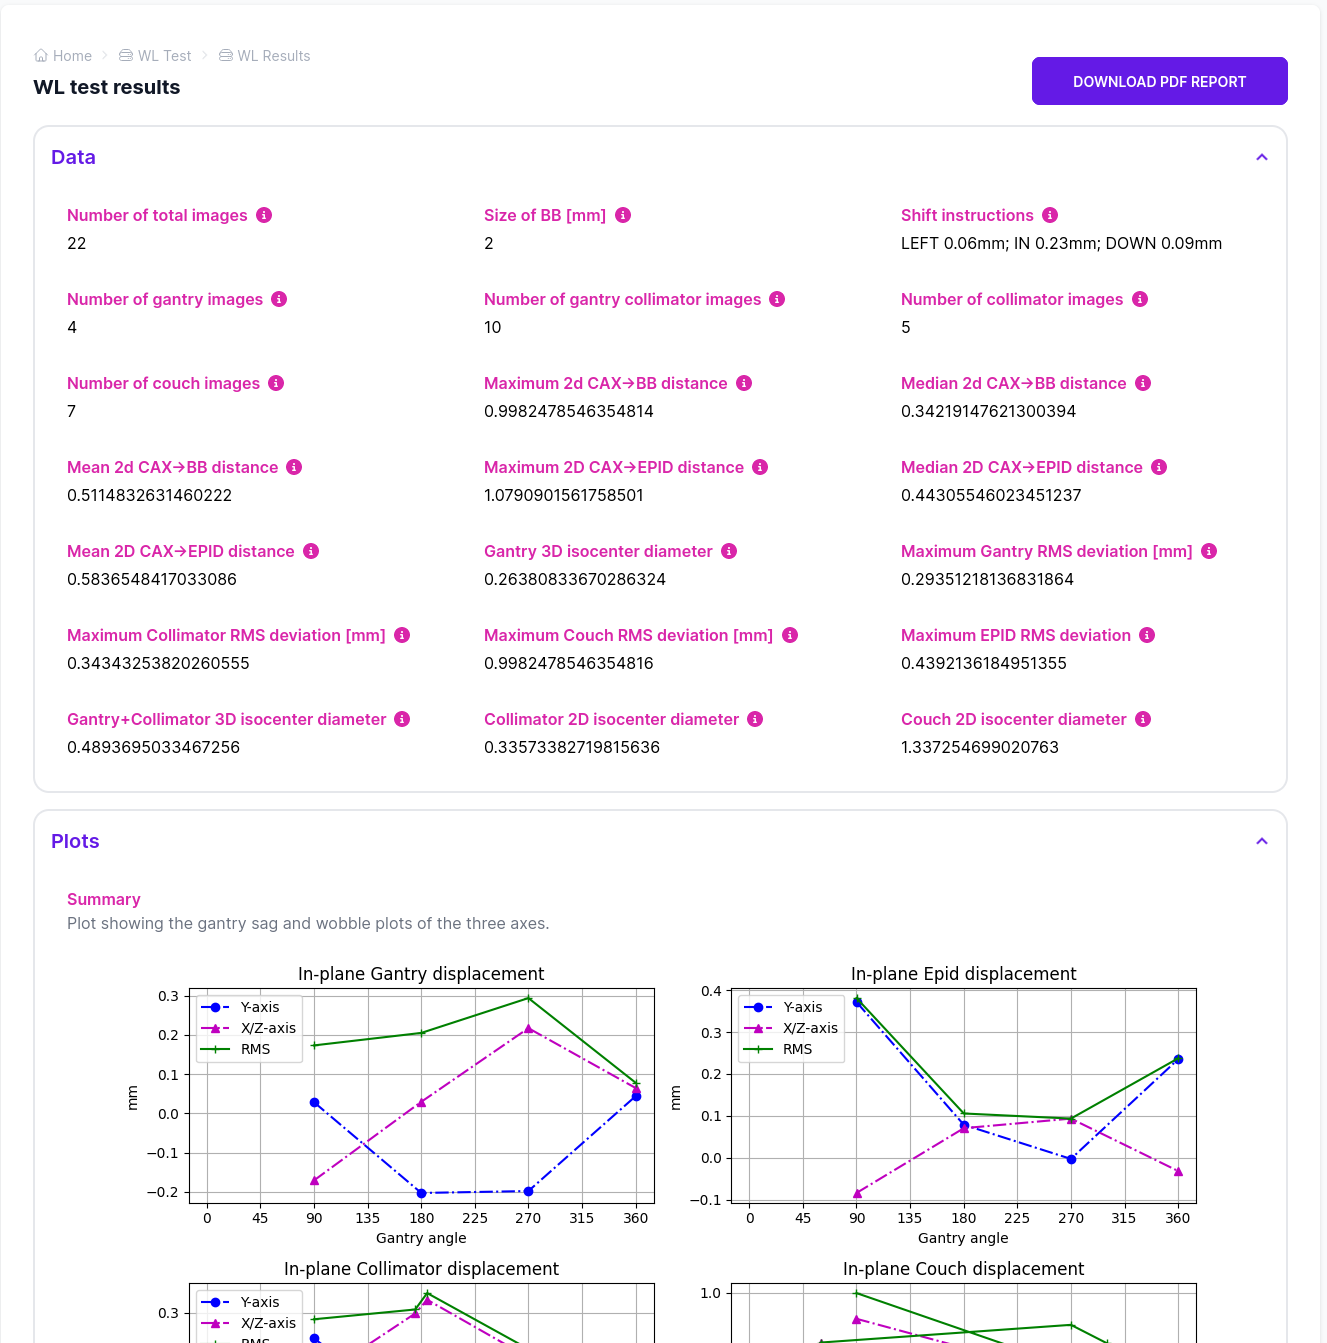
\includegraphics[width=1\textwidth]{Content/Images/ui_wl_results_page.png}
    \caption{W-L test results page}
    \label{fig:uiWLResults}
\end{figure}

\subsubsection{LA analysis setup page}

LA analysis setup page consists of eight numerical inputs and two file selectors. Files for this module are uploaded via the existing common file upload interface for the entire application. Interface is shown in \autoref{fig:uiLACommonFileUpload}.

Once all the fields have been filled in and the files selected, a preview of the preprocessed will be available. This allows the parameters of the algorithm to be adjusted so that the edges of the radiation field are correctly detected. LA setup page is shown on \autoref{fig:uiLASetup}.

\begin{figure}
    \centering
    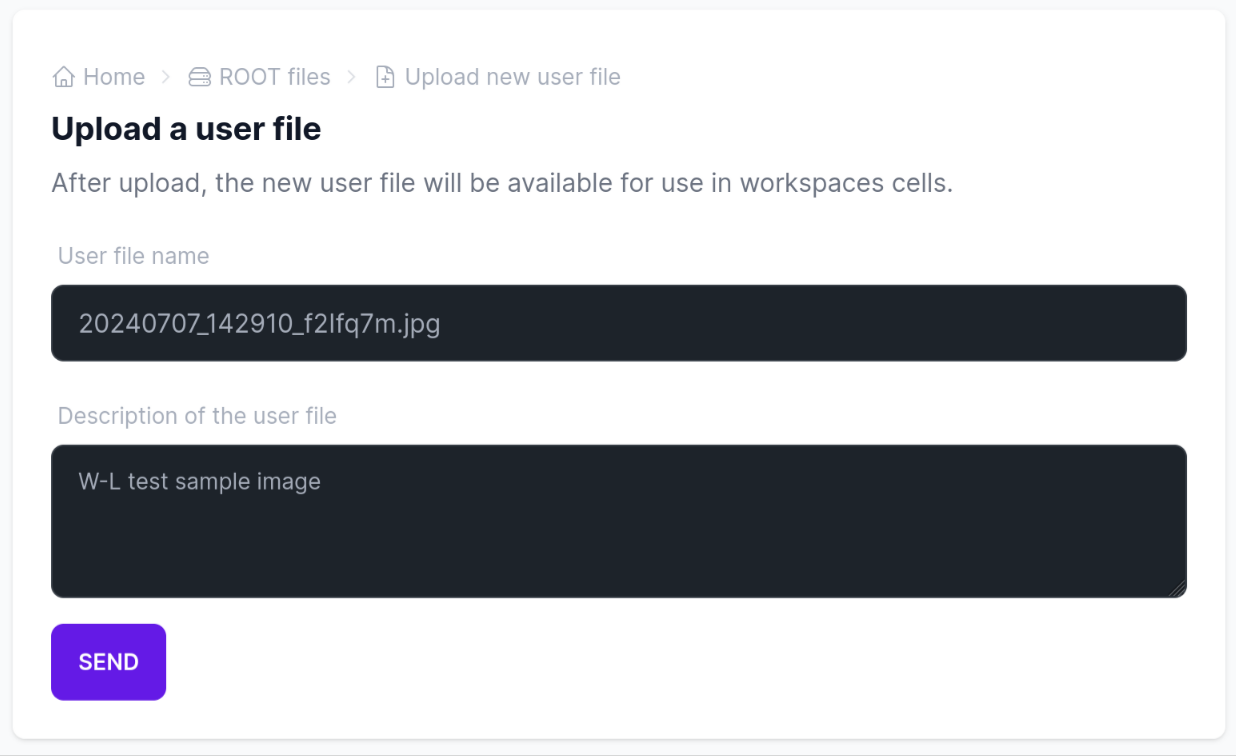
\includegraphics[width=0.8\textwidth]{Content/Images/ui_la_upload.png}
    \caption{Common interface for uploading files}
    \label{fig:uiLACommonFileUpload}
\end{figure}

\begin{figure}
    \centering
    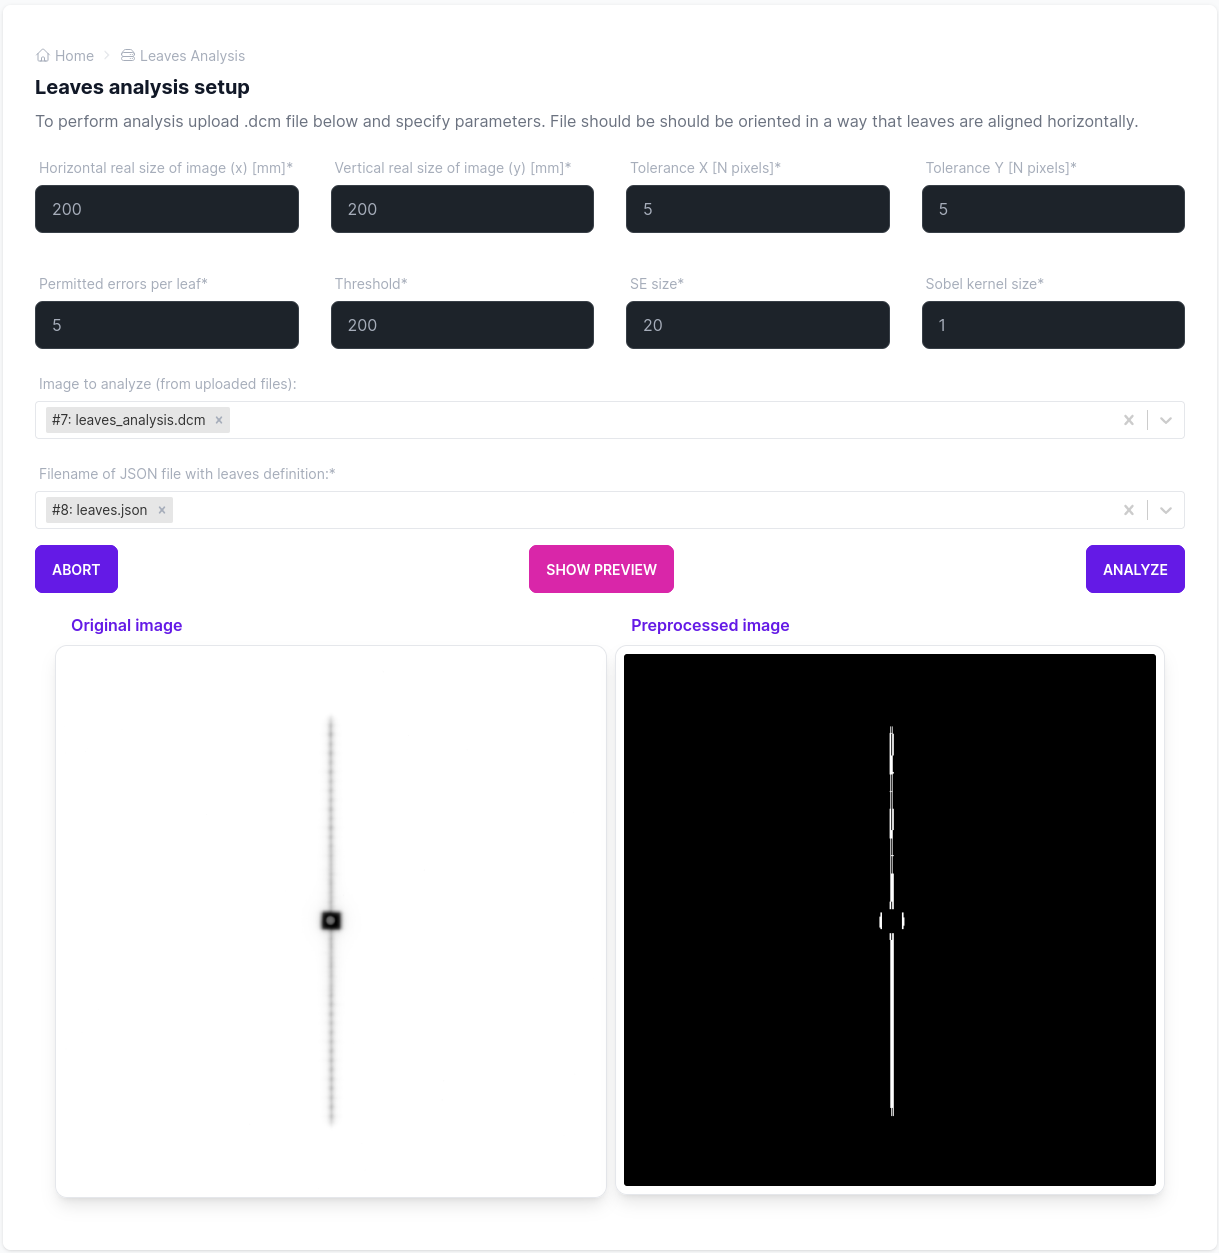
\includegraphics[width=1\textwidth]{Content/Images/ui_la_setup_page.png}
    \caption{LA analysis setup page}
    \label{fig:uiLASetup}
\end{figure}

\subsubsection{LA analysis results page}

The results page shows the original image, the preprocessed image, the resulting image for the left leaves and the resulting image for the right leaves.

A list of faulty leaves is listed below on the left. On the right-hand side, a legend for the colours can be found.

In the top left-hand corner of the page, there is a toggle switch which, when clicked on, brings up the visualisation of the leaves on all 4 images. LA analysis results page can be found on \autoref{fig:uiLAResults}.

\begin{figure}
    \centering
    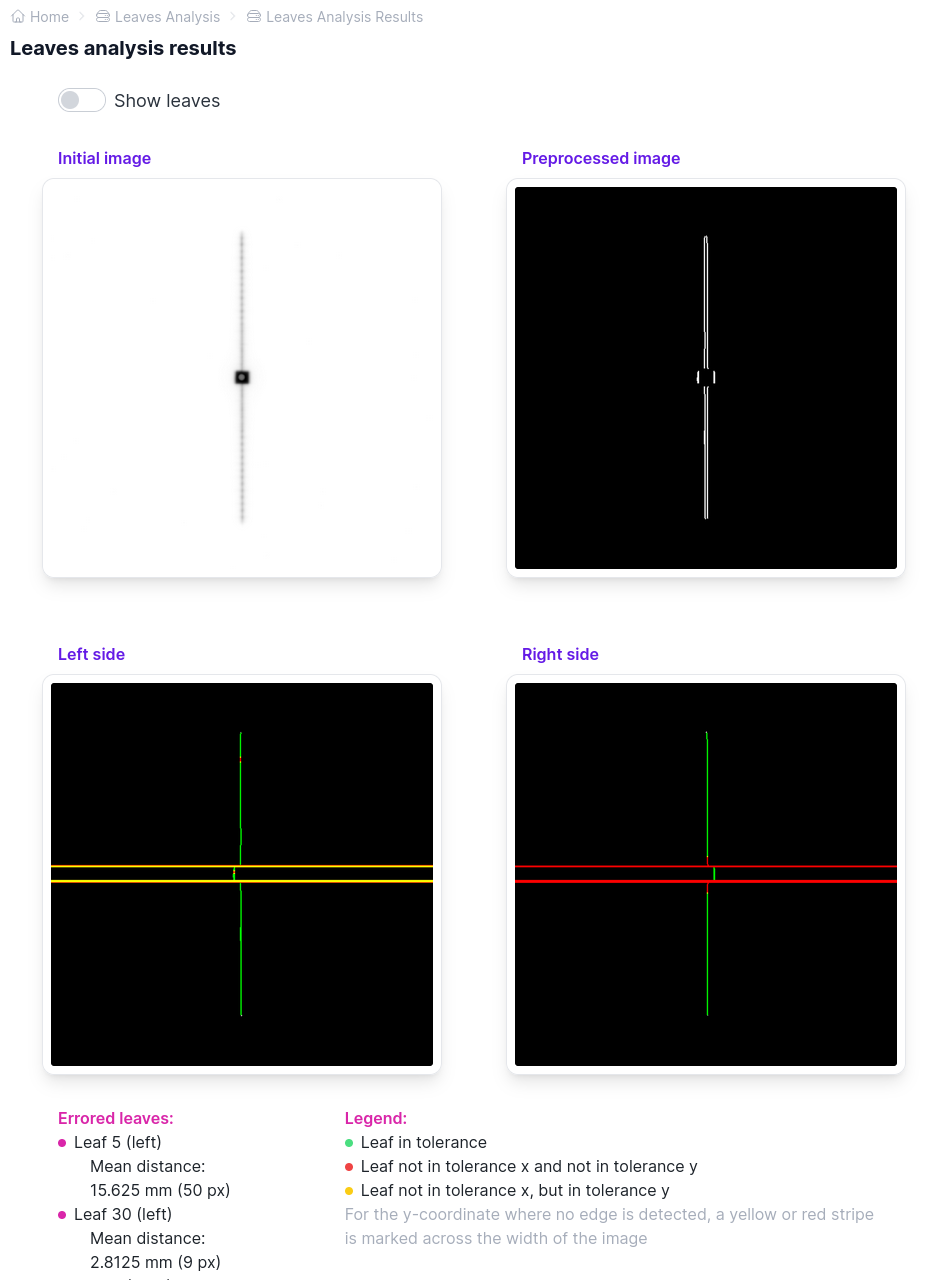
\includegraphics[width=1\textwidth]{Content/Images/ui_la_results_page.png}
    \caption{LA analysis results page}
    \label{fig:uiLAResults}
\end{figure}

\subsection{Implementation}

\subsubsection{W-L Test}

The setup component contains forms with one numerical-only field and a second file field that uploads the file to the server. The file is hashed to save space and data and cache the data for results. If there is the same file already present on the server it is overwritten. BB size and filename are sent as a parameter to the results page.

The result page component has 3 separate React Query hooks that separately fetch numeric data, plots and pdfs, to speed up loading. Once loaded, each element is displayed independently of the others. The data is cached and the key consists of filename and BB size, with a stale time of 5 minutes. Therefore, if the user executes a query with the same parameters within 5 minutes, the data is loaded from the cache and is displayed immediately without the need to make another request to the backend.

\subsubsection{LA analysis}

On the setup page, there are eight fields in which only numbers can be entered. Furthermore, there are two fields for selecting files that have previously been uploaded via the common interface. After selecting a file, the server is queried and returns the names of the uploaded files, which are then displayed as options to the user.

When the \verb|show preview| button is clicked, a request to the backend is made, and the server returns a pre-processed image. As with the W-L test, it is cached, with the test parameters being the keys. This means that if a user switches back to the previously used parameters, the preview images will be loaded immediately from the cache. In contrast to the \verb|show preview| button, which does not switch pages, clicking on the \verb|analyze| button will take the user to the results page.

As LA analysis does not take long, the results page contains only one React Query hook. The server then returns the data, along with two variants of the images - with and without leaves drawn. When the toggle is clicked, the images are replaced on the frontend without additional requests to the server.

\section{Backend}
\label{sec:techWL}
\label{sec:techLA}

\subsection{Structure}

The modules have been added to the application in a separate folder \verb|contrib|. The LA analysis module is more straightforward and consists of a \verb|views.py| file with two views that manage the endpoints defined below and a second file with algorithm definitions.

W-L module also includes analogous \verb|views.py| file and algorithm declarations files, as well as \verb|models.py|, \verb|serializer.py| and \verb|utils.py| files. These files are responsible for handling uploads that overwrite files with the same name to optimize storage.

Additionally, both modules contain a \verb|apps.js| file, which is a required component in the Django framework for applications located in separate folders.

\subsection{API}

\subsubsection{W-L Test}

Four endpoints are available in this module. 2 of them return data about the W-L test, and they have been split to enable independent data loading on frontend - text data, that loads faster, can be displayed earlier, and plots can be loaded in parallel.

\paragraph{Endpoints}

\begin{itemize}
    \item \verb|/api/wl/text/|

    Endpoint for fetching text data results of W-L test.

    Type: GET
    
    Request payload: Filename and BB size.
    
    Response payload: All numerical data of W-L test as defined in \autoref{sec:wlTestNumericalOutput}
    
    \item \verb|/api/wl/plots/|
    
    Endpoint for fetching plots of W-L test.

    Type: GET
    
    Request payload: Filename and BB size.
    
    Response payload: Zip file with plot of isocenter visualisation and summary plot.
    
    \item \verb|/api/wl/pdf/|

    Endpoint for downloading PDF report.

    Type: GET
    
    Request payload: Filename and BB size.
    
    Response payload: PDF file with results of W-L test.
    
    \item \verb|/api/wl/upload/|

    Endpoint for uploading images that will be used in the W-L test.

    Type: POST
    
    Request payload: Zip file with W-L EPID images. 
    
    Response payload: Status of operation.
    
\end{itemize}

\subsubsection{LA Analysis}

Two endpoints are available in this module, one for the preprocessing of images and a second for full LA analysis.

\paragraph{Endpoints}

\begin{itemize}
    \item \verb|/api/la/preprocess/|

    Endpoint for fetching preprocessed images.

    Type: GET
    
    Request payload: Filename of image to analyze, binarization threshold, structuring element size, Sobel kernel size.
    
    Response payload: Zip file with original image and image after preprocessing (\autoref{sec:laDetermineEdgesAlgorithm})
    
    \item \verb|/api/la/analyze/|
    
    Endpoint for fetching result images.

    Type: GET
    
    Request payload: All inputs defined in \autoref{sec:laAnalysisInputs}.
    
    Response payload: All outputs defined in \autoref{sec:laAnalysisOutputs}. Images are zipped into the zip file.
    
\end{itemize}